
\section{Automate à états finis en découlant}

De ces diagrammes de séquence découlent quelques questions primaires qui ont dû être traités en tout premier lieu, avant encore d'entamer la conception de notre programme, à commencer par sa représentation 'graphique'. Le schéma suivant montre le modèle final de notre programme ainsi que tous ses états et transitions possibles.\\


\begin{figure}[!ht]
	\center
	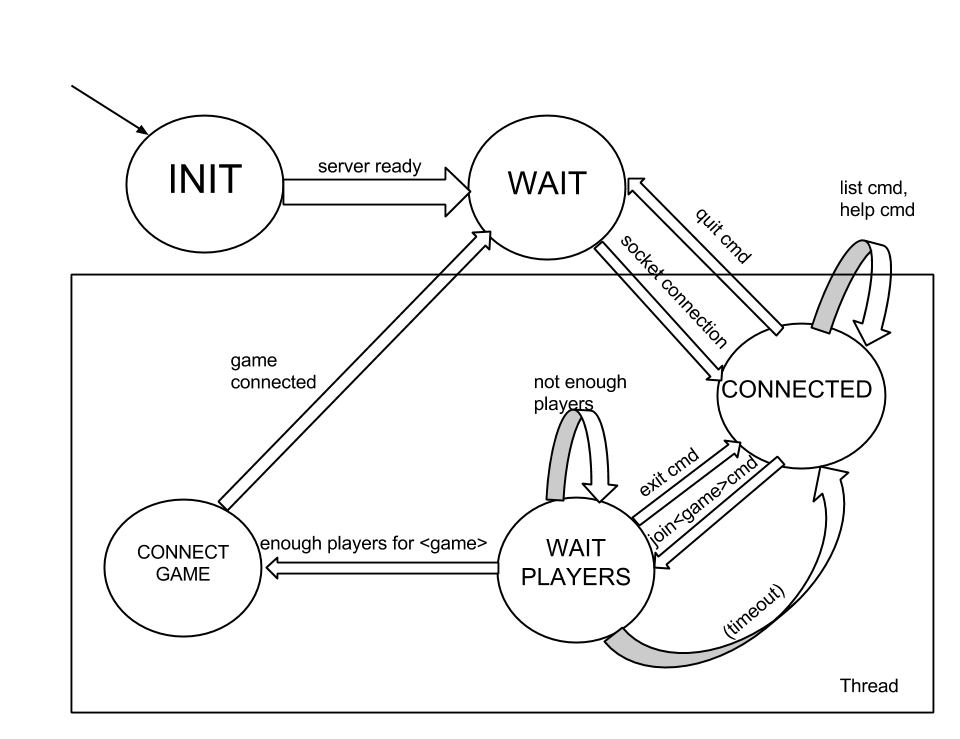
\includegraphics[scale=0.5]{images/state_machine_server.png}
	\caption{L'automate décrivant notre serveur}
\end{figure}


\underline{Explication}\\


\begin{itemize}
	\item \textbf{INIT}\\
	La phase d'initialisation du serveur, qui devrait être plus ou moins instantanée.
	\vspace{1em}
	
	
	\item \textbf{WAIT}\\
	Une fois l'initialisation terminée et le serveur prêt, celui-ci entre dans une phase d'attente, où il attendra la connexion d'un client. Dans le cadre de ce projet, le client est une simple application développée en parallèle, mais à l'avenir, le logiciel est prévu pour soutenir n'importe quel type de client.
	\newpage
	
	
	\item \textbf{CONNECTED}\\
	Le client, une fois connecté, est en mesure d'envoyer des commandes et en recevoir les réponses. Le format utilisé est le JSON, pour la compréhension sur multiples supports et son universalité.
	Si l'utilisateur entre les commandes 'list' ou 'help', il reste dans l'état courant, CONNECTED. Il ne changera d'état qu'à deux conditions:
	
	\begin{itemize}
		\item La commande 'quit', pour se déconnecter du service
		\item La commande 'join (game)' afin de d'accéder au service principal du serveur, soit la connexion à un jeu.
	\end{itemize}
	\vspace{1em}
	
	
	\item \textbf{WAIT PLAYERS}\\
	Cet état est un état intermédiaire entre l'envoi de la commande et la connexion effective au jeu demandé. En effet, on ne peut se connecter à jeu que sous certaines conditions:
	\begin{itemize}
		\item Il y a déjà une ou plusieurs instances du jeu demandé en cours, et il y a des places restantes pour y jouer -au cas où ils ont plus de deux joueurs-.
		\item Il y a assez de joueurs demandant le jeu pour instancier une nouvelle partie.
	\end{itemize}
	\vspace{1em}
	
	En dehors de ces deux conditions, le client restera dans cet état. Si l'attente est trop longue, le client est renvoyé dans l'état précédent, pouvant alors demander un autre jeu ou retenter une connexion / une instanciation du jeu existant.
	\vspace{1em}
	
	
	\item \textbf{CONNECT GAME}\\
	Une fois que l'une ou l'autre de ces conditions sont réunies, le client peut enfin se voir connecter à l'instance d'une partie ou la créer avec un autre joueur, et ainsi y jouer. Dès lors, le rôle du serveur est terminé, et il retourne dans l'état \textbf{WAIT} pour qu'un autre client s'y connecte.
	
	
\end{itemize}

\vspace{6em}
Ainsi défini, nous avons un cadre clair et des états définis auxquels s'en tenir lors de notre développement: notre ligne de conduite est désormais claire pour le développement de ce serveur, nous pouvons nous pencher sur les aspects plus techniques de ce projet, posant les problématiques et y donnant des éléments de réponse à intégrer dans notre logiciel.
